%-------------------------------------------------------------------------------
\section{Answer Set Programming}
%-------------------------------------------------------------------------------
\label{sec:asp}

The concretization problem is essentially a combinatorial search problem. While many
package managers use homegrown SAT solvers for this type of problem, encoding the
complexity of our domain in pure Boolean SAT would be extremely tedious. To manage the
complexity, we leverage Answer Set Programming (ASP), a form of declarative programming
that allows us to formally specify our semantics in first-order logic with variables and
quantification, in addition to Boolean operators. The input language for ASP is similar
to Prolog~\cite{baral_2003}. Unlike Prolog, ASP has no operational semantics and is not
Turing-complete. Rather, ASP converts first-order logic programs (with quantifiers and
variables) to {\it propositional} programs (with no variables). It then uses techniques
borrowed from SAT solvers to find solutions. One major benefit of this approach is that
unlike Prolog, ASP programs are guaranteed to terminate.

In the remainder of this section, we illustrate how ASP can simplify the specification
and maintenance of our concretization algorithm while also affording strong guarantees
than we can implement ourselves with simple heuristics.

\subsection{ASP Syntax}

ASP programs are comprised of ``terms'', which can be Boolean atoms or a functions whose
arguments may also be terms. A term followed by a period ({\tt .}) is called a ``fact''.
The following is a simple program comprised entirely of facts:
\begin{minted}[fontsize=\small, bgcolor=bg]{prolog}
  optimize_for_reuse.
  node("hdf5").
  depends_on("hdf5", "mpi").
\end{minted}
Note that these functions are not imperative; rather this snippet can be ready roughly
as ``{\tt optimize\_for\_reuse} is enabled. A node called {\tt hdf5} exists. {\tt hdf5} depends on {\tt mpi}.''

In addition to facts, ASP programs contain rules, which can derive additional facts. An
ASP rule has a {\it head} and a {\it body}, separated by \texttt{:-}. The \texttt{:-}
can be read as ``if'' --- the head (left side) is true {\it if} the body (right side) is true.
Terms in the body of a rule can also be preceded by the keyword ``not'' to imply the
head based on their negation. Logical ``and'' is represented by a comma in the rule
body, and ``or'' is represented by repeating the head with a different rule body.

ASP programs can contain variables, represented by capitalized words. Variables are
scoped to the rule or fact in which they appear; the variable {\tt Package} may be used
in unrelated rules without any scoping issues. Rules are instantiated with all possible
substitutions for variables. For example:
%Additionally, variables appearing in the
%head of a rule must appear in a positive (non-negated) term in the rule body. This is
%referred to as ``safety'' in ASP, and is essential to ensuring the algorithm will
%terminate.
\begin{minted}[fontsize=\small, bgcolor=bg]{prolog}
  node("hdf5").
  depends_on("hdf5", "mpi").
  node(Dependency) :-
      node(Package), depends_on(Package, Dependency).
\end{minted}
The rule here translates roughly to ``If a package is in the graph and it depends on
another package, that package must be in the graph'', and the rule in the program above
will derive the fact {\tt node("mpi")} when it is instantiated with {\tt
  node("hdf5")} and {\tt depends\_on("hdf5", "mpi")}. This is the essence of how
  we model dependencies in ASP.

\subsection{Integrity Constraints and Choices}

Two additional types of rules are important to understand the power of ASP:
\textit{integrity constraints} and \textit{choice rules}.
%Answer Set Programming gets its name from the set of possible answers which satisfy the constraints of the program.
%ASP solvers focus on understanding the constraints on this space.
Integrity constraints allow the programmer to rule out swathes of the answer set space
by specifying conditions not to allow. In ASP, these are represented by a headless rule:
\begin{minted}[fontsize=\small, bgcolor=bg]{prolog}
  node("hdf5").
  depends_on("hdf5", "mpi").
  node(Dependency) :-
      node(Package), depends_on(Package, Dependency).
  :- depends_on(Package, Package).
\end{minted}
This constraint says ``a package cannot depend on itself''.

\subsection{Choice Rules}

Choice rules give the solver freedom to choose from possible options. A choice rule is
(optionally) constrained on either side to specify the minimum (left) and maximum
(right) number of choices the solver can select.
\begin{minted}[fontsize=\small, bgcolor=bg]{prolog}
  node("hdf5").
  depends_on("hdf5", "mpi").
  node(Dependency) :-
      node(Package), depends_on(Package, Dependency).
  :- depends_on(Package, Package).

  possible_version("hdf5", "1.13.1").
  possible_version("hdf5", "1.12.1").
  1 { version(P, V) : possible_version(P, V) } 1 :-
      node(P).
\end{minted}
The choice rule on the last line means ``If a package is in the graph, assign it
exactly one of its possible versions.'' The $\{a:b\}$ syntax here has the same meaning
as in formal set theory; it denotes the set of all $a$ such that $b$ is true. The
numerals on either side of the choice rule are {\it cardinality constraints}; they specify
lower and upper bounds on the size of the set. Choice rules are similar to guessing;
they give the solver options for paths to explore next.

%allow the solver substantial freedom to create facts, within the specified
%constraints, that satisfy other constraint of the program or maximize optimization
%criteria.

\subsection{Optimization}

In addition to constraints on the solution space, ASP allows optimization criteria.
Optimization criteria allow the solver to return a single answer set from the among all
valid answer sets, and they guarantee that the chosen answer set minimizes or maximizes one
or many criteria. There are often many valid solutions to a dependency resolution query,
but only the optimal solution is relevant once we find it.
\begin{minted}[fontsize=\small, bgcolor=bg]{prolog}
  node("hdf5").
  depends_on("hdf5", "mpi").
  node(Dependency) :-
      node(Package), depends_on(Package, Dependency).
  :- depends_on(Package, Package).

  possible_version("hdf5", "1.13.1", 0).
  possible_version("hdf5", "1.12.1", 1).

  1 { version(P, V) : possible_version(P, V) } 1 :-
      node(P).

  version_weight(P, V, Weight) :-
      possible_version(P, V, Weight).
  #minimize{ W@3,P,V : version_weight(P, V, W)}.
\end{minted}
This optimization constraint says ``I prefer (at priority 3) solutions that minimize the
sum of the weights ({\tt W}) of the package ({\tt P}) versions ({\tt V}), for all
packages and versions.'' A detailed discussion of the syntax for optimization is beyond
the scope of this paper; it suffices to know that multi-objective optimization across a
variety of criteria is possible in ASP.

Our small and very incomplete program here already shows the power of ASP. In a SAT
solver, the programmer would need to write out explicitly the rule for deriving
dependency nodes from dependent nodes for every possible pair of packages. Even worse,
our choice rule for selecting versions would need to be written out for every
combination of package and version, and an enormous combination of logical operators
constructed to ensure that for any group of versions \texttt{$a_1, ..., a_n$}, one of
the constructions \texttt{$a_i$} and not any \texttt{$a_j$} for all $i\neq{j}$. ASP
makes this much simpler.

%Writing
%out the facts of our small program in SAT is hard enough, and we haven't even discussed
%implementing optimization criteria in Boolean logic. In ASP, though, it appears
%reasonably straightforward and is legible to future maintainers of our code.

\subsection{Grounding and Solving}

ASP solvers search the input program for {\it stable models}, also known as
\textit{answer sets}. An answer set is a set of true atoms for which every rule in the
input program is idempotent. It is similar to a fixed point, or the solution to a system
of (Boolean) equations. When ASP first emerged in the late 1990's, it used custom solvers.
However, the problem domain of ASP is NP-complete, and the 2000's brought great
advances~\cite{moskewicz2001chaff} in solving the canonical NP-complete problem: Boolean
satisfiability (SAT). Modern ASP solvers exploit high-performance techniques developed
in the SAT community~\cite{gebser+:asp-book}.

\begin{figure*}[t]
  \centering
  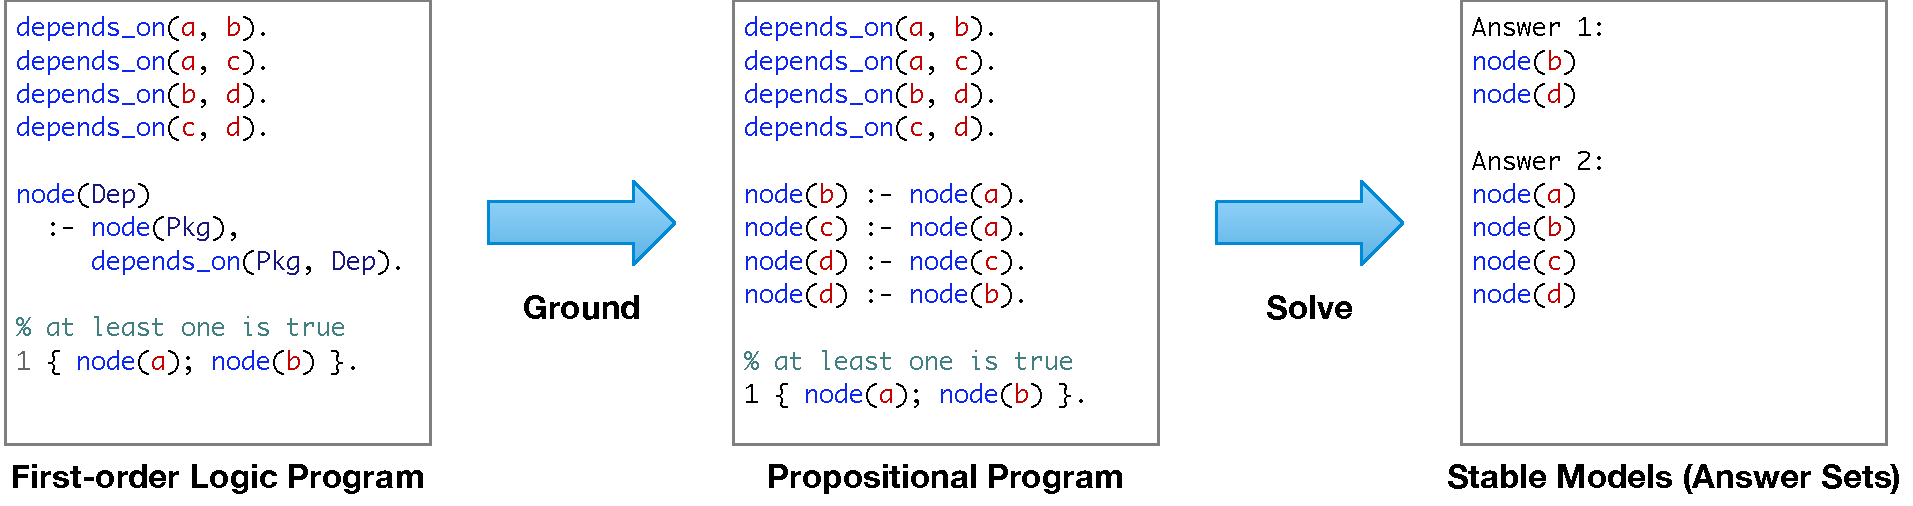
\includegraphics[width=.8\textwidth]{figures/asp-grounding.pdf}
  \caption{
    Grounding and solving in Answer Set Programming.
    \label{fig:ground-solve}
    \vspace{-1em}
  }
\end{figure*}

The ASP input language, with first-order rules and variables, is very expressive, but
SAT solvers deal with {\it propositional} logic programs that have no variables. A logic
expression that has no variables is called a {\it ground} term, and {\it grounding} is
the process of converting a first-order ASP rules to a set of ground rules. We call
these the ``ground instances'' of the rule.

Figure~\ref{fig:ground-solve} shows the grounding and solving process at a very high
level. On the left is an ASP program with four facts, one first-order rule, and a choice
rule that says we must choose at least one of {\tt node(a)} or {\tt node(b)} to be in
the solution. Grounding this program {\it instantiates} the first-order rule with all
possible ground atoms that can be substituted into its body. The ground instances are
built from input {\tt depends\_on()} facts, {\tt node(a)} and {\tt node(b)} from the
choice rule, as well as {\tt node(c)} and {\tt node(d)}, which appear in the heads of
ground rules instantiated from {\tt node(a)} and {\tt node(b)}. Note that the ground
instances are simplified---they omit {\tt depends\_on()} terms because these are facts
in the input, and therefore always true. Grounders perform many such optimizations to
prune the propositional program and to make the solver more efficient.

Propositional logic programs can be reduced to SAT and solved using techniques similar
to those used in modern SAT solvers~\cite{gebser+:asp-book}. For this program, there are
two stable models: one with only {\tt node(b)} and {\tt node(d)} (when only {\tt
  node(b)} is selected by the choice rule) and one with all four nodes (when only {\tt
  node(a)} or both {\tt node(a)} and {\tt node(b)} are selected). It is easy to see from
this result how we could read in these lists of nodes and construct graphs from them.
This how Spack reads solutions in from the solver.

We use the popular {\tt clingo}~\cite{gebser+:aicomm11} system, which includes a
grounder ({\tt gringo}) and a solver ({\tt clasp}). The search algorithm used in {\tt
  clasp} traces its roots to the well known Davis–Putnam–Logemann–Loveland (DPLL)
algorithm~\cite{dp-sat,dpll-sat}, but uses modern extensions like Conflict-Driven Clause
Learning (CDCL) for high performance~\cite{moskewicz2001chaff}. {\tt clasp} can also
do MaxSAT-style optimization.
%\texttt{gringo} ``grounds'' the first-order input problem to produce the
%propositional form accepted by {\tt clasp}.
%
The internals of {\tt clingo} are beyond the scope of this paper, but is important to
understand that because it effectively performs an exhaustive combinatorial search, it
guarantees completeness and optimality. There are no inputs for which {\tt clingo} will
return a false negative (claim compatible rules are incompatible) and solutions
are guaranteed to be optimal according to provided criteria.
